\documentclass{llncs}
%\pagestyle{headings} %page numbers
%\usepackage[font=small,labelfont=bf]{caption}


%% Language and font encodings
\usepackage[english]{babel}
\usepackage[utf8x]{inputenc}
\usepackage[T1]{fontenc}
\usepackage[outdir=./]{epstopdf}
\usepackage{bm}

\usepackage[]{xcolor}
%% Sets page size and margins
\usepackage[a4paper,top=3cm,bottom=2cm,left=3cm,right=3cm,marginparwidth=1.75cm]{geometry}

%% Useful packages
%\usepackage{amsmath}
\usepackage{graphicx}

\usepackage[colorinlistoftodos]{todonotes}
\title{Super awesome embeddings}
\author{Grzegorz Beringer \and Mateusz Jabłoński \and Piotr Januszewski \and Julian Szymański}
%

 \institute{
Faculty of Electronic Telecommunications and Informatics\\
Gda{\'n}sk University of Technology, Gda{\'n}sk, Poland
}

% (feature abused for this document to repeat the title also on left hand pages)

% the affiliations are given next; don't give your e-mail address
% unless you accept that it will be published
%\institute{Faculty of Electronics,
%Telecommunications and Informatics,
%Gdańsk University of Technology,
%ul. Narutowicza 11/12, 80-952 Gdańsk,
%Poland}

\begin{document}
\maketitle
\begin{abstract}
Abstract
\keywords{word sense disambiguation, word embeddings}

\end{abstract}

\section{Introduction}
\label{introduction}

Word Sense Disambiguation (WSD) is an open problem of natural language processing (NLP) and ontology. WSD is identifying which sense of a word (i.e. meaning) is used in a sentence based on the word context. Difficulty is when the word has multiple meanings (e.g. a decision tree, a tree data structure, a tree in a forest). The problem requires two inputs: a dictionary to specify the senses which are to be disambiguated and a corpus of language data to be disambiguated. WSD task has two variants: "lexical sample" and "all words" task. The former aim to disambiguate the occurrences of a small sample of selected target words, while in the latter all the words in a piece of running text need to be disambiguated. Our solution targets the former one, but could be extended to the latter variant.
The solution to WSD would be useful in many NLP related problems as: relevance of search engines, anaphora resolution, coherence, inference, etc.

Word embeddings are a product of feature learning techniques in NLP, where words from the vocabulary are mapped to vectors of real numbers. Conceptually it involves a dimensionality reduction from a space with one dimension per word to a continuous vector space with a much lower dimension.
Methods to generate this mapping include artificial neural networks\cite{word2vec}\cite{GloVe}\cite{fastText}, dimensionality reduction on the word co-occurrence matrix\cite{Levy2014NWE} and probabilistic models\cite{Globerson2007EEC}.
Word embeddings are commonly used as the input representation. They have been shown to boost the performance in NLP tasks such as syntactic parsing\cite{parsingGrammars} and sentiment analysis\cite{sentimentAnalysis}.

Word embeddings cannot distinguish between different meanings of ambiguous words by themselves. By definition, there is only one embedding for each word e.g. for word ``tree'' there is a single real-valued vector. What can be done, is to try to distinguish the meaning based on the context, in which the word was used. Then, we treat each meaning as a separate keyword, which has its own embedding.
We propose a simple method to infer the word meaning: an average of the context and the word embeddings and number of improvements to this approach in the chapter ``Our method''. Experiments with our solution are presented in the chapter ``Experiments''. To conduct those experiments we have created the dataset composed of 6 ambiguous words, with 4 to 7 meanings each, and collected real-world usage examples of those meanings, with tagged words to be disambiguated. We describe our dataset in the chapter ``Dataset''. In the chapter ``Related work'' we present other approaches to WSD.

\section{Related work}
\label{related work}

Typically, there are two kinds of approach for WSD: supervised, which make use of sense-annotated training data, and knowledge-based, which make use of the properties of lexical resources. In supervised approach, the most widely used training corpus used is SemCor\cite{semcor}, with 226,036 sense annotations from 352 manually annotated documents.
Knowledge-based systems usually exploit WordNet\cite{wordnet} or BabelNet\cite{babelnet} as semantic network.
Our solution joins two approaches. We use the knowledge-based word embeddings like GloVe\cite{GloVe} as a baseline for our method and then optimize them in supervised fashion.

The most usual baseline is the Most Frequent Sense\cite{evalmfs} (MFS) heuristic, which selects for each target word the most frequent sense in the training data.
Recent growth of sequence learning techniques using artificial neural networks contributed to WSD research: Raganato et al.\cite{neuralseqmodelingforWSD} propose a series of end-to-end neural architectures directly tailored to the task, from bidirectional Long Short-Term Memory (LSTM) to encoder-decoder models. Melamud et al.\cite{context2vec} also use bidirectional LSTM it their work. They use large plain text corpora to learn a neural model that embeds entire sentential contexts and target words in the same low-dimensional space, which is optimized to reflect inter-dependencies between targets and their entire sentential context as a whole.

Iacobacci et al.\cite{embeddingsforWSD} were first to try to use word embeddings for WSD. They consider four different strategies for integrating a pre-trained word embeddings as context representation in a supervised WSD system: concatenation, average, fractional and exponential decay of the vectors of the words surrounding a target word.
Peters et al.\cite{deepcontext} create word representations that differ from traditional word embeddings in that each token is assigned a representation that is a function of the entire input sentence. They use vectors derived from a bidirectional LSTM that is trained with a coupled language model objective on a large text corpus.

Most of the previous neural networks applications to WSD ignore lexical resources like glosses (sense definitions) and rely solely on word's context. In Luo et al.\cite{glosses} paper, they integrate the context and glosses of the target word into a unified framework, in order to make full use of both labeled data and lexical knowledge.

Entity Linking (EL) and WSD both address the lexical ambiguity of language. The aim of EL is to discover mentions of entities within text and to link them to the most suitable entry in a reference knowledge base. The two tasks are pretty similar, but they differ fundamentally: in EL the textual mention can be linked to a named entity which may or may not contain the exact mention, while in WSD there is a perfect match between the word form and a suitable word sense in the knowledge base.
Moro et al.\cite{babelfy} present Babelfy, a unified graph-based approach to EL and WSD based on a loose identification of candidate meanings coupled with a densest subgraph heuristic, which selects high-coherence semantic interpretations.
We can find also application of random walks\cite{randomwalks} and topic models\cite{topicmodels} for knowledge-based WSD.

Developing WSD system requires much effort and as a result, very few open source WSD systems are publicly available. Zhong et al.\cite{itmakessense} present an English all-words WSD system, IMS (It Makes Sense), built using a supervised learning approach that is written in Java and completely open source. Following Lee and Ng\cite{SVMtoWSD}, they adopt support vector machines (SVM) as the classifier and integrate multiple knowledge sources including parts-of-speech (POS), surrounding words, and local collocations as features.

\section{Dataset}
\label{dataset}
For the purpose of testing word embeddings as a method to differentiate between different meanings, we gathered examples for 6 ambiguous words, 4-7 meanings each (28 meanings in total).
Ambiguous word together with its meaning constitues a \textit{keyword}, which we use as a separate class when identyfing the closest meaning given some context.
All keywords can be seen on Figure 1.

\begin{figure}
    \label{fig:keywords}
    \caption{Ambiguous words with their meanings (keywords) from the dataset}
    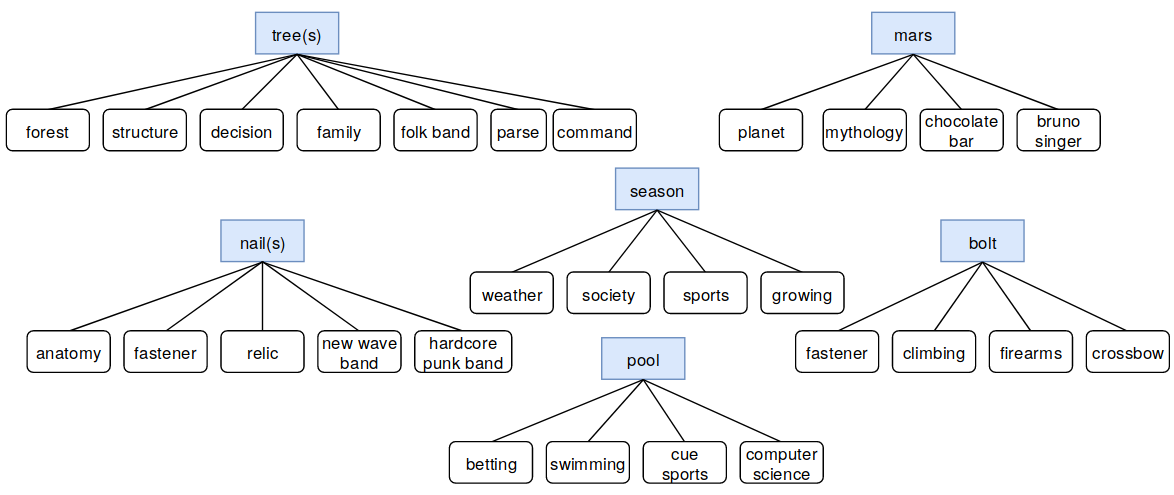
\includegraphics[scale=0.35]{res/keywords.png}
\end{figure}

Examples were mostly gathered from Wikipedia, using \textit{What links here} utility for each keyword.
If usage examples from Wikipedia were not enough, other websites were used (or even the Wikipedia article on specific keyword itself).

The dataset is split into training and test set, with 5 training and 10 test examples for each keyword.
Each example is stored in plain text, with the ambiguous word marked with "*" on both sides.

The correct keyword for each example, together with a path to file and a link, where the original text was taken from, are stored in CSV files: \textit{train.csv} for training set, \textit{test.csv} for test set (columns: path,keyword,link).
Keywords themselves, together with links to their Wikipedia articles, are stored in \textit{keywords.csv} file.
Dataset, together with the code to execute experiments from this paper, can be found on our GitHub repository \cite{repository}.

\bigskip
\underline{Example for \textit{bolt crossbow} keyword:}

\smallskip
\textbf{Keyword definition}: keyword.csv\newline
\textit{
keyword,link\newline
...\newline
bolt crossbow,https://en.wikipedia.org/wiki/Crossbow\_bolt}

\smallskip
\textbf{Test set}: test.csv\newline
\textit{
path,keyword,link\newline
...\newline
texts/test/bolt\_crossbow\_5.txt,bolt crossbow,https://en.wikipedia.org/wiki/Incendiary\_device
}

\smallskip
\textbf{Text}: texts/test/bolt\_crossbow\_5.txt\newline
\textit{"Sulfur- and oil-soaked materials were sometimes ignited and thrown at the enemy, or attached to spears, arrow and *bolts* and fired by hand or machine. Some siege techniques—such as mining and boring—relied on combustibles and fire to complete the collapse of walls and structures."}

\section{Our method}
\subsection{Keyword embedding}
\textit{Keyword} is a sequence of words that lets us disambiguate between different meanings of the same ambiguous word, e.g. "tree forest" that represents a tree as a plant and "tree structure" which represents tree as a mathematical structure.

To get the embedding of the keyword, we simply average all the words in the keyword:

\begin{equation}
    \label{eq:keyword_embedding}
    \bm{k} = e(w_1, w_2, ..., w_N) = \frac{1}{N}\sum_{i=1}^{N} e(w_i)
\end{equation}

where \(e(\cdot)\) is the embedding function used and \(w_1, w_2, ..., w_N\) is a sequence of N words that, in this case, constitutes a keyword.

\subsection{Context embedding}
\textit{Context} is a sequence of words that contains an ambiguous word within, usually in the middle.
It is parametrized by context length \(l\), which specifies how many of words from both side of the ambiguous word in question were taken into consideration.

\textit{Context embedding} \(\bm{c}\) is also achieved by taking an average of word embeddings (Equation \ref{eq:keyword_embedding}).
In this case, \(N = 2l + 1\) and \(w_1, w_2, ..., w_N\) is the context with ambiguous word inside. For some cases \(N < 2l + 1\), since the ambiguous word may occur at the beginning or ending of text example and full context cannot be collected.
In this case, we just average the reduced context.

Text, that we take context from, must be preprocessed.
We remove any special characters and stopwords, and use lower-case letters only.

\underline{Example with \(l=3\)}:

\textbf{Text}:
\textit{"The object pool pattern is a software creational design pattern that uses a set of initialized objects kept ready to use – a " *pool* " – rather than allocating and destroying them on demand."}

\textbf{Preprocessed text}:
\textit{"the object pool pattern is a software creational design pattern that uses a set of initialized objects kept ready to use a *pool* rather than allocating and destroying them on demand"}

\textbf{Context}:
\textit{kept ready use \underline{pool} rather allocating destroying}

\subsection{Optimization}
As a baseline, we use keyword and context embeddings described above to find the closest keyword given some context, using cosine distance as a metric.
To optimize this system, we use texts from the training set to improve the quality of keyword embeddings.
For each training example, we shift the correct keyword embedding by a factor of \(\alpha\) in the direction of context embedding, which describes said keyword.

\begin{equation}
    \label{eq:alpha_optimization}
    \bm{k}^{(i+1)} = \bm{k}^{(i)} + \alpha(\bm{c} - \bm{k}^{(i)})
\end{equation}

where \(\bm{k}^{(i)}\) is the embedding of the correct keyword at iteration \(i\), \(\bm{c}\) is the context embedding and \(\alpha\) is a scalar that controls the strength of the update.

\smallskip
We try to optimize the system even further, by also moving top-k closest keywords that are incorrect given the same context.

\begin{equation}
    \label{eq:beta_optimization}
    \bm{m}^{(i+1)} = \bm{m}^{(i)} - \beta(\bm{c} - \bm{m}^{(i)})
\end{equation}

where \(\bm{m}^{(i)}\) is the embedding of incorrect keyword at iteration \(i\) and \(\beta\) is a scalar that controls the strength of the update.

\section{Experiments}
\subsection{Assumptions}
Since our goal is to check how embedding approach works for WSD problem, we use pretrained embedding model from spaCy - en\_vectors\_web\_lg.
Due to high impact of training data order on test results, as a result we take average score of 30 runs for each optimization.
\subsection{Baseline}
First of experiments is to check how out-of-the-box model works without extra optimizations. We perform tests with different context lengths, as a score we choose top 1 and top 3 accuracy. Results are shown in the Fig. \ref{fig:baseline}.

\begin{figure}
    \label{fig:baseline}
    \caption{Top accuracy of base model with different context length}
    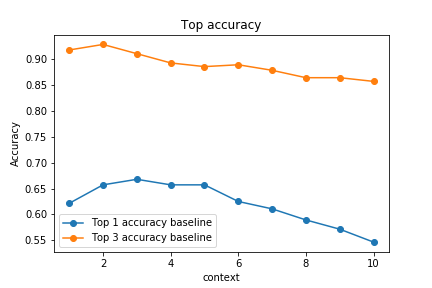
\includegraphics[scale=0.5]{res/baseline_context_top_acc.png}
\end{figure}
TODO: Some discussion.
\subsection{Context length optimization}
Once we have base model results we check how simple alpha optimization improves accuracy based on context length. To do this, we choose arbitrarily a value for alpha parameter and run tests after one epoch of training the model. Since we average results from 30 runs we mark the measurement uncertainty on the graph. Results are shown in the Fig. \ref{fig:exp1}.
\begin{figure}
    \label{fig:exp1}
    \caption{Comparison of the base model and a little bit optimized model based on different context length}
    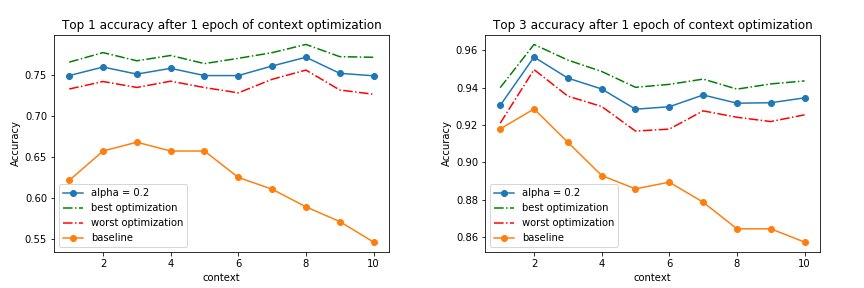
\includegraphics[scale=0.6]{res/exp1_context_top_acc.png}
\end{figure}
TODO: Some discussion.

\subsection{Alpha parameter optimization}
Next step is to check the influence of alpha parameter on the accuracy score after one epoch of training with fixed context length - the best value for the base model. Results are shown in the Fig. \ref{fig:exp2}. In this experiment we also mark the measurement uncertainty on the graph.

\begin{figure}
    \label{fig:exp2}
    \caption{Based on fixed context length, comparison of the base model and a model optimized with various alpha parameters. }
    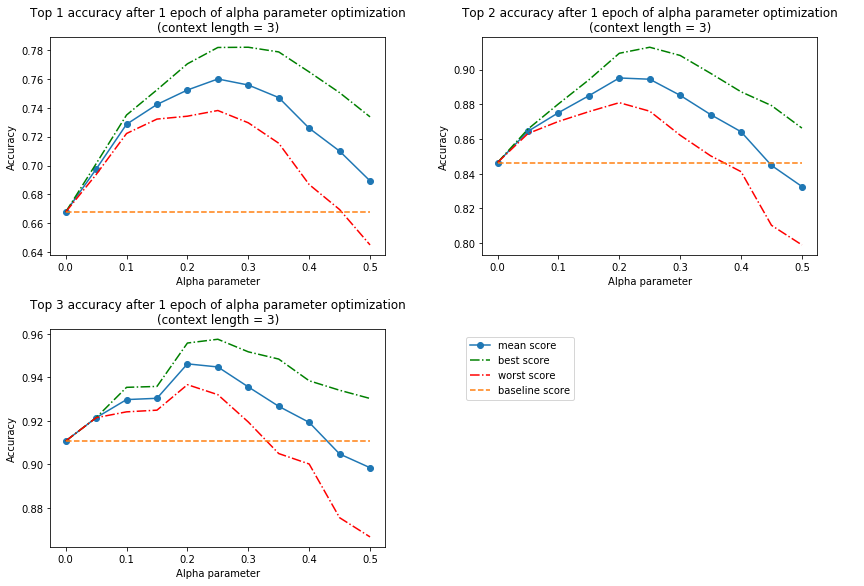
\includegraphics[scale=0.6]{res/exp2_alpha_top_acc.png}
\end{figure}
TODO: Some discussion.
\subsection{Beta parameter optimization}
Next optimization we test is the influence of beta parameter. In this test we also performs one epoch of training with fixed context length and alpha parameter, based on previous experiment's results. Results are shown in the Fig. \ref{fig:exp3}. Since in this case we compare our solution to non-fully deterministic solution we decide to mark only averaged score of performed tests.

\begin{figure}
    \label{fig:exp3}
    \caption{Based on fixed context length and alpha parameter value, comparison of the alpha-optimized model and a alpha-optimized model with various beta parameters. }
    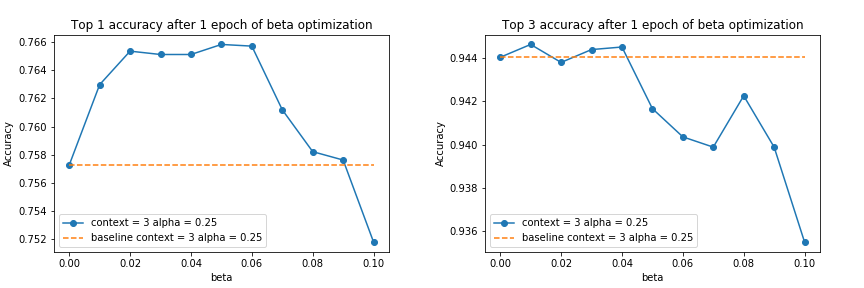
\includegraphics[scale=0.5]{res/exp3_beta_top_acc.png}
\end{figure}
TODO: Some discussion.

\subsection{Longer training}
Previous optimization are applied for only one epoch of training. The goal of next experiment is to check how number of epochs affects final accuracy. We run up to 5 epochs of training using parameters obtained in previous experiments. Results are shown in the Fig. \ref{fig:exp4_2}.
\begin{figure}
    \label{fig:exp4_1}
    \caption{5 epoch training of optimized model}
    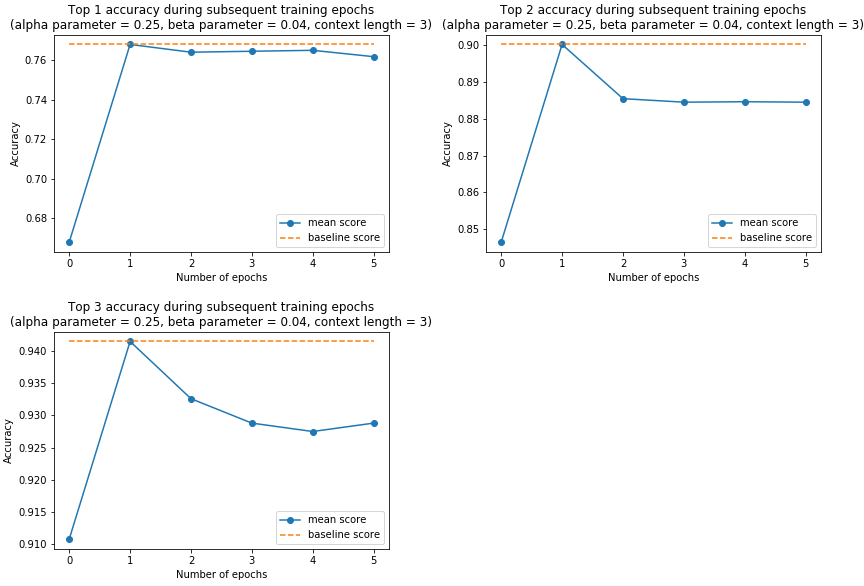
\includegraphics[scale=0.6]{res/exp4_epoch_top_acc.png}
\end{figure}
We see that there is almost no improvement after first epoch of training. Probably the problem is that alpha and beta parameters are too big. We also check what happens when we choose lower values of alpha/beta parameters. Results are shown in the Fig. \ref{fig:exp4_2}.
\begin{figure}
    \label{fig:exp4_2}
    \caption{Comparison of multiple optimized models across 5 epochs of training. }
    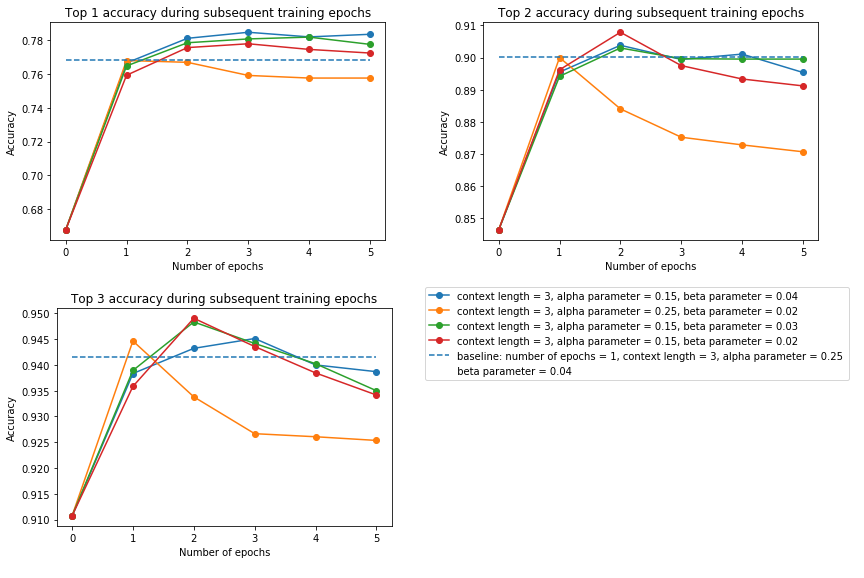
\includegraphics[scale=0.6]{res/exp4_epoch_multiconfiguration_top_acc.png}
\end{figure}
TODO: Some discussion.

\bibliographystyle{splncs}
\bibliography{sample}

\end{document}


\begin{thebibliography}

\end{thebibliography}
